%  LaTeX support: latex@mdpi.com 
%  For support, please attach all files needed for compiling as well as the log file, and specify your operating system, LaTeX version, and LaTeX editor.

%=================================================================
%\documentclass[journal,article,submit,moreauthors,pdftex]{Definitions/mdpi}
\documentclass[preprints,article,accept,moreauthors,pdftex]{Definitions/mdpi} 

% For posting an early version of this manuscript as a preprint, you may use "preprints" as the journal and change "submit" to "accept". The document class line would be, e.g., \documentclass[preprints,article,accept,moreauthors,pdftex]{mdpi}. This is especially recommended for submission to arXiv, where line numbers should be removed before posting. For preprints.org, the editorial staff will make this change immediately prior to posting.

%--------------------
% Class Options:
%--------------------
%----------
% journal
%----------
% Choose between the following MDPI journals:
% acoustics, actuators, addictions, admsci, adolescents, aerospace, agriculture, agriengineering, agronomy, ai, algorithms, allergies, analytica, animals, antibiotics, antibodies, antioxidants, appliedchem, applmech, applmicrobiol, applnano, applsci, arts, asi, atmosphere, atoms, audiolres, automation, axioms, batteries, bdcc, behavsci, beverages, biochem, bioengineering, biologics, biology, biomechanics, biomedicines, biomedinformatics, biomimetics, biomolecules, biophysica, biosensors, biotech, birds, bloods, brainsci, buildings, businesses, cancers, carbon, cardiogenetics, catalysts, cells, ceramics, challenges, chemengineering, chemistry, chemosensors, chemproc, children, civileng, cleantechnol, climate, clinpract, clockssleep, cmd, coatings, colloids, compounds, computation, computers, condensedmatter, conservation, constrmater, cosmetics, crops, cryptography, crystals, curroncol, cyber, dairy, data, dentistry, dermato, dermatopathology, designs, diabetology, diagnostics, digital, disabilities, diseases, diversity, dna, drones, dynamics, earth, ebj, ecologies, econometrics, economies, education, ejihpe, electricity, electrochem, electronicmat, electronics, encyclopedia, endocrines, energies, eng, engproc, entropy, environments, environsciproc, epidemiologia, epigenomes, fermentation, fibers, fire, fishes, fluids, foods, forecasting, forensicsci, forests, fractalfract, fuels, futureinternet, futuretransp, futurepharmacol, futurephys, galaxies, games, gases, gastroent, gastrointestdisord, gels, genealogy, genes, geographies, geohazards, geomatics, geosciences, geotechnics, geriatrics, hazardousmatters, healthcare, hearts, hemato, heritage, highthroughput, histories, horticulturae, humanities, hydrogen, hydrology, hygiene, idr, ijerph, ijfs, ijgi, ijms, ijns, ijtm, ijtpp, immuno, informatics, information, infrastructures, inorganics, insects, instruments, inventions, iot, j, jcdd, jcm, jcp, jcs, jdb, jfb, jfmk, jimaging, jintelligence, jlpea, jmmp, jmp, jmse, jne, jnt, jof, joitmc, jor, journalmedia, jox, jpm, jrfm, jsan, jtaer, jzbg, kidney, land, languages, laws, life, liquids, literature, livers, logistics, lubricants, machines, macromol, magnetism, magnetochemistry, make, marinedrugs, materials, materproc, mathematics, mca, measurements, medicina, medicines, medsci, membranes, metabolites, metals, metrology, micro, microarrays, microbiolres, micromachines, microorganisms, minerals, mining, modelling, molbank, molecules, mps, mti, nanoenergyadv, nanomanufacturing, nanomaterials, ncrna, network, neuroglia, neurolint, neurosci, nitrogen, notspecified, nri, nursrep, nutrients, obesities, oceans, ohbm, onco, oncopathology, optics, oral, organics, osteology, oxygen, parasites, parasitologia, particles, pathogens, pathophysiology, pediatrrep, pharmaceuticals, pharmaceutics, pharmacy, philosophies, photochem, photonics, physchem, physics, physiolsci, plants, plasma, pollutants, polymers, polysaccharides, proceedings, processes, prosthesis, proteomes, psych, psychiatryint, publications, quantumrep, quaternary, qubs, radiation, reactions, recycling, regeneration, religions, remotesensing, reports, reprodmed, resources, risks, robotics, safety, sci, scipharm, sensors, separations, sexes, signals, sinusitis, smartcities, sna, societies, socsci, soilsystems, solids, sports, standards, stats, stresses, surfaces, surgeries, suschem, sustainability, symmetry, systems, taxonomy, technologies, telecom, textiles, thermo, tourismhosp, toxics, toxins, transplantology, traumas, tropicalmed, universe, urbansci, uro, vaccines, vehicles, vetsci, vibration, viruses, vision, water, wevj, women, world 

%---------
% article
%---------
% The default type of manuscript is "article", but can be replaced by: 
% abstract, addendum, article, book, bookreview, briefreport, casereport, comment, commentary, communication, conferenceproceedings, correction, conferencereport, entry, expressionofconcern, extendedabstract, datadescriptor, editorial, essay, erratum, hypothesis, interestingimage, obituary, opinion, projectreport, reply, retraction, review, perspective, protocol, shortnote, studyprotocol, systematicreview, supfile, technicalnote, viewpoint, guidelines, registeredreport, tutorial
% supfile = supplementary materials

%----------
% submit
%----------
% The class option "submit" will be changed to "accept" by the Editorial Office when the paper is accepted. This will only make changes to the frontpage (e.g., the logo of the journal will get visible), the headings, and the copyright information. Also, line numbering will be removed. Journal info and pagination for accepted papers will also be assigned by the Editorial Office.

%------------------
% moreauthors
%------------------
% If there is only one author the class option oneauthor should be used. Otherwise use the class option moreauthors.

%---------
% pdftex
%---------
% The option pdftex is for use with pdfLaTeX. If eps figures are used, remove the option pdftex and use LaTeX and dvi2pdf.

%=================================================================
% MDPI internal commands
\firstpage{1} 
\makeatletter 
\setcounter{page}{\@firstpage} 
\makeatother
\pubvolume{1}
\issuenum{1}
\articlenumber{0}
\pubyear{2021}
\copyrightyear{2020}
%\externaleditor{Academic Editor: Firstname Lastname} % For journal Automation, please change Academic Editor to "Communicated by"
\datereceived{} 
\dateaccepted{} 
\datepublished{} 
\hreflink{https://doi.org/} % If needed use \linebreak
%------------------------------------------------------------------
% The following line should be uncommented if the LaTeX file is uploaded to arXiv.org
\pdfoutput=1

%=================================================================
% Add packages and commands here. The following packages are loaded in our class file: fontenc, inputenc, calc, indentfirst, fancyhdr, graphicx, epstopdf, lastpage, ifthen, lineno, float, amsmath, setspace, enumitem, mathpazo, booktabs, titlesec, etoolbox, tabto, xcolor, soul, multirow, microtype, tikz, totcount, changepage, paracol, attrib, upgreek, cleveref, amsthm, hyphenat, natbib, hyperref, footmisc, url, geometry, newfloat, caption

\usepackage{amsmath}


%----------------MACROS--------------------
\def\github{\url{https://github.com/anthony-walker/pysweep-git}}
\def\pysweep{\texttt{PySweep}}
\def\Swept{\texttt{Swept}}
\def\Standard{\texttt{Standard}}
\def\Up{\texttt{Up-Pyramid}}
\def\Down{\texttt{Down-Pyramid}}
\def\Oct{\texttt{Octahedron}}
\def\Xb{\texttt{X-Bridge}}
\def\Yb{\texttt{Y-Bridge}}
\newcommand\fs{0.7}

\def\oldCPU{Intel Skylake Silver 4114} %20 core cpu
\def\oldGPU{Nvidia GeForce GTX 1080 Ti}

\def\newCPU{Intel E5-2698v4} %20 core cpu
\def\newGPU{Nvidia Tesla V100-DGXS-32GB}

%=================================================================
%% Please use the following mathematics environments: Theorem, Lemma, Corollary, Proposition, Characterization, Property, Problem, Example, ExamplesandDefinitions, Hypothesis, Remark, Definition, Notation, Assumption
%% For proofs, please use the proof environment (the amsthm package is loaded by the MDPI class).

%=================================================================
% Full title of the paper (Capitalized)
\Title{The Two-Dimensional Swept Rule Applied on Heterogeneous Architecture}

% MDPI internal command: Title for citation in the left column
\TitleCitation{The Two-Dimensional Swept Rule Applied on Heterogeneous Architecture}

% Author Orchid ID: enter ID or remove command
\newcommand{\orcidauthorA}{0000-0002-0616-6998} % Add \orcidA{} behind the author's name
\newcommand{\orcidauthorB}{0000-0003-4425-7097} % Add \orcidB{} behind the author's name

% Authors, for the paper (add full first names)
\Author{Anthony Walker\orcidA{} and Kyle E.~Niemeyer\orcidB{}}

% MDPI internal command: Authors, for metadata in PDF
\AuthorNames{Anthony Walker and Kyle E.~Niemeyer}

% MDPI internal command: Authors, for citation in the left column
\AuthorCitation{Walker, A.; Niemeyer, K.E.}
% If this is a Chicago style journal: Lastname, Firstname, Firstname Lastname, and Firstname Lastname.

% Affiliations / Addresses (Add [1] after \address if there is only one affiliation.)
\address[1]{%
School of Mechanical, Industrial, and Manufacturing Engineering\\
Oregon State University\\
Corvallis, Oregon, USA}

% Contact information of the corresponding author
\corres{Correspondence: kyle.niemeyer@oregonstate.edu}

% % Current address and/or shared authorship
% \firstnote{Current address: Affiliation 3} 
% \secondnote{These authors contributed equally to this work.}
% % The commands \thirdnote{} till \eighthnote{} are available for further notes

%\simplesumm{} % Simple summary

%\conference{} % An extended version of a conference paper

% Abstract (Do not insert blank lines, i.e. \\) 
\abstract{The partial differential equations describing compressible fluid flows can be notoriously difficult to resolve on a pragmatic scale and often require the use of high performance computing systems and/or accelerators. 
However, these systems face scaling issues such as latency, the fixed cost of communicating information between devices in the system. The swept rule is a technique designed to minimize these costs by obtaining a solution to unsteady equations at as many possible spatial locations and times prior to communicating. 
In this study, we implemented and tested the swept rule for solving two-dimensional problems on heterogeneous computing systems across two distinct systems. Our solver showed a speedup range of 0.22--2.71 for the heat diffusion equation and 0.52--1.46 for the compressible Euler equations. 
We can conclude from this study that the swept rule offers both potential for speedups and slowdowns and that care should be taken when designing such a solver to maximize benefits. These results can help make decisions to maximize these benefits and inform designs.}

% Keywords
\keyword{Latency; GPU; CPU; PDE} 

% The fields PACS, MSC, and JEL may be left empty or commented out if not applicable
%\PACS{J0101}
%\MSC{}
%\JEL{}

%%%%%%%%%%%%%%%%%%%%%%%%%%%%%%%%%%%%%%%%%%
% Only for the journal Diversity
%\LSID{\url{http://}}

%%%%%%%%%%%%%%%%%%%%%%%%%%%%%%%%%%%%%%%%%%
% Only for the journal Applied Sciences:
%\featuredapplication{Authors are encouraged to provide a concise description of the specific application or a potential application of the work. This section is not mandatory.}
%%%%%%%%%%%%%%%%%%%%%%%%%%%%%%%%%%%%%%%%%%

%%%%%%%%%%%%%%%%%%%%%%%%%%%%%%%%%%%%%%%%%%
% Only for the journal Data:
%\dataset{DOI number or link to the deposited data set in cases where the data set is published or set to be published separately. If the data set is submitted and will be published as a supplement to this paper in the journal Data, this field will be filled by the editors of the journal. In this case, please make sure to submit the data set as a supplement when entering your manuscript into our manuscript editorial system.}

%\datasetlicense{license under which the data set is made available (CC0, CC-BY, CC-BY-SA, CC-BY-NC, etc.)}

%%%%%%%%%%%%%%%%%%%%%%%%%%%%%%%%%%%%%%%%%%
% Only for the journal Toxins
%\keycontribution{The breakthroughs or highlights of the manuscript. Authors can write one or two sentences to describe the most important part of the paper.}

%%%%%%%%%%%%%%%%%%%%%%%%%%%%%%%%%%%%%%%%%%
% Only for the journal Encyclopedia
%\encyclopediadef{Instead of the abstract}
%\entrylink{The Link to this entry published on the encyclopedia platform.}
%%%%%%%%%%%%%%%%%%%%%%%%%%%%%%%%%%%%%%%%%%

\begin{document}

\section{Introduction}
Partial differential equations (PDEs) are used to model many important phenomena in science and engineering. Among these, fluid mechanics and heat transfer are which can be notoriously difficult to solve on pragmatic scales. Wildfire is a good example of an expensive numerical simulation because it involves fluid mechanics, heat transfer, and chemical reactions over massive areas of impact. Wildfire is also an unsteady phenomenon---so it changes over time. The ability to accurately model and predict the properties of such phenomena in real time would allow for better responses, but there are many challenges associated with making these predictions.

Unsteady multi-dimensional PDEs often require using of distributed-memory computing systems to obtain a solution with practical grid resolution or scale in a reasonable time frame. Advancing the solution at any point in the grid inherently depends on the neighboring points in each spatial dimension. This dependence requires communication between computing nodes, to transfer data associated with the boundary locations. Each of these communications incurs a minimum cost regardless of the amount of information communicated---this is network latency. In contrast, bandwidth is the variable cost associated with the amount of data transferred. The total latency cost can significantly restrict the solution's time to completion, especially when using distributed systems. This barrier to scaling is referred to as the "latency barrier" and is impacts large-scale simulations that involve advancing many time steps, i.e., ones that require a large amount of communication \cite{Alhubail2016ThePDEs}. The barrier is a bottle neck in the system which can limit the performance regardless of the architecture.

\par
Graphics processing units (GPUs) are powerful tools for scientific computing because they are well suited for parallel applications and large quantities of simultaneous calculations. Modern computing clusters often have GPUs in addition to CPUs because of their potential to accelerate simulations and, similar to CPUs, they perform best when communication is minimized. These modern clusters are often referred to as heterogeneous systems or systems with multiple processor types---CPUs and GPUs, in this case. Ideally, a heterogeneous application will minimize communication between the GPU and CPU which effectively minimizes latency costs \cite{OanceaGPGPUCOMPUTING}. Minimizing latency in high performance computing is one of the barriers to exascale computing which requires the implementation of novel techniques to improve \cite{Alexandrov2016RouteSkills}.

\par
   This study presents our implementation and testing of a two-dimensional heterogeneous solver for unsteady partial differential equations that employs a technique to help overcome the latency barrier---the swept rule \cite{Alhubail2016ThePDEs}. In other words, the swept rule is a latency reduction technique that focuses on obtaining a solution to unsteady PDEs at as many possible locations and times prior to communicating with other computing nodes (ranks). In this article, we first discuss related work, distinguish our work from prior swept studies, and provide more motivation in section~\ref{related-section}. Next, we describe implementation details, objectives, study parameters, design decisions, methods, and tests in section~\ref{methods-section}. As expected, this is followed with results and conclusions in sections~\ref{results-section} and~\ref{conclusions-section}.

\label{related-section}
\par Surmounting the latency barrier has been approached in many ways; the most closely related to this study include prior swept rule studies which involve multiple dimensions and architectures but not the combination of the two \cite{Alhubail2016ThePDEs,Alhubail2018ThePDEs,Magee2018AcceleratingDecomposition,Magee2020ApplyingSystems}. Parallel-in-time methods are also related to the swept rule but differ in the sense that they iteratively parallelize the temporal direction, while the swept rule minimizes communication \cite{Gander201550Integration}. There are many examples of parallel-in-time methods which are all variations of the core concept \cite{Falgout2014ParallelMultigrid,Lions2013Resolution,Maday2020AnAlgorithm,Wu2018Parareal,EmmettTowardEquations,MinionINTERWEAVINGMULTIGRID,Hahne2020PyMGRIT:MGRIT}. For example, Parareal is one of the more popular parallel-in-time methods; it works by iterating over a series of coarse and fine grids with initial guesses to parallelize the problem \cite{Lions2013Resolution}. However, there are some stability concerns with Parareal that are addressed by local time integrators \cite{Wu2018Parareal}. These methods have the same goal but achieve that goal differently. Similarly, cache optimization techniques have the same objective, but they achieve it differently by optimizing communication not avoiding it \cite{Kowarschik2003AnAlgorithms}.

\par
 Finally, communication avoidance techniques closely emulate the swept rule but involve overlapping parts or redundant operations. The GPU implementation particularly blurs this difference because it solves an extra block to avoid intra-node communication but no extra blocks are solved for inter-node communication. The swept rule also differs because it particularly focuses on solving PDEs. There are varying degrees of communication algorithms that tend to focus on linear algebra \cite{DemmelAvoidingComputations, Ballard2011MinimizingAlgebra,BaboulinAMachines,Khabou2012LUVersion,SolomonikAHoefler}. 

\par
The swept rule was originally developed by Alhubail et al \cite{Alhubail2016ThePDEs}. who first developed a one-dimensional CPU-only swept PDE solver which was tested by solving the Kuramoto-Sivashinsky equation and the compressible Euler equations. They concluded that in each case a number of integrations can be performed during the latency time of a communication. Their analysis showed that integration can be made faster by latency reduction and increasing computing power of the computing nodes \cite{Alhubail2016ThePDEs}. Alhubail et al. followed this work with a two-dimensional CPU only swept PDE solver which reported speedups of up to three times compared to classical methods when solving the wave and Euler equations \cite{Alhubail2018ThePDEs}. These studies differ from our study most prominently by the dimensionality and intended architecture.

\par
Magee et al. created a one-dimensional GPU swept solver and a one-dimensional heterogeneous solver and applied both to solving the compressible Euler equations \cite{Magee2018AcceleratingDecomposition,Magee2020ApplyingSystems}. They concluded that their shared memory approach typically performed better than alternative approaches, but speedup was not obtained in all cases for either study. Varying performance results were attributed to greater usage of lower-level memory, which limits the performance benefits of the swept rule depending on the problem \cite{Magee2018AcceleratingDecomposition}. Our current study extends upon the swept rule for heterogeneous architectures, but it differs in the dimensionality. Our implementation also attempts to use and extend some of the implementation strategies that showed promise in the aforementioned studies.

\par
The effect of added dimensionality on performance is a pragmatic interest and can be considered from multiple perspectives. The primary goal is speeding up simulations requiring high performance computing by reducing network latency. The swept rule is motivated by reducing the time to obtain solutions of problems involving complicated phenomena frequently requiring the use of high performance computing systems. While many simplifications exist to reduce the dimensionality of fluid dynamics problems, most realistic problems are three-dimensional. Our solver is a step towards more realistic simulations by considering two spatial dimensions, which can provide insight into multi-dimensional performance and constraints. This insight can offer the chance to optimize system usage and promote faster design and prototype of thermal fluid systems.

\par
In the event that computation time is not the primary concern, available resources or resource costs are important considerations. The ability to execute a simulation on a high performance computing system depends on access to such systems. Pay per use systems like Amazon AWS, Microsoft Azure, and Google Cloud offer cloud computing time. However, pricing models for university-managed clusters remain ambiguous making determination of cost challenging on the user's end \cite{Mesnard2019}. In the case of Amazon EC2, simulation time can be purchased at different hourly rates depending on the application. We generated an estimate using Amazon's pricing tool with a two node configuration (\texttt{g4dn.xlarge} instances) which yielded a monthly "on-demand" cost of \$928.46 \cite{AmazonServices}. Purchasing such time and configures quickly becomes expensive for applications that require large numbers of computing hours or larger hardware configurations. Network latency contributes substantially to this cost as it is aggrandized in applications requiring a lot of communication because each communication event takes a finite amount of time regardless of the data size. 

Furthermore, it is possible to obtain and show performance benefits on smaller systems. This claim is supported by findings from Magee et al.; they showed speedup on a work station with a single GPU and CPU \cite{Magee2018AcceleratingDecomposition}. While this is not the primary focus, an optimized solver that reduces latency would require less computing resources and more practical applications could potentially be solved on smaller, less costly computing clusters. Hopefully, it is clear at this point that latency reduction is important in high performance computing and scientific applications as this is the intention of this work.


%%%%%%%%%%%%%%%%%%%%%%%%%%%%%%%%%%%%%%%%%%
\section{Materials and Methods}
\label{methods-section}
\subsection{Implementation \& Objectives}
We call our implementation of the two-dimensional swept rule \pysweep{}\footnote{\pysweep is openly available at \github}---it consists of two core solvers: \Swept{} and \Standard{}. \Swept{} minimizes communication during the simulation via the swept rule. \Standard{} is a traditional solver that communicates as is necessary to complete a timestep, and serves as a baseline to the swept rule. Both solver use the same decomposition, process handling, and work allocation code so that a performance comparison between them is representative of swept rule performance. However, \Swept{} does require additional calculations prior to solving which are penalties of this swept rule implementation. 

\par
We implemented \pysweep{} using Python and CUDA; the parallelism relies primarily on \texttt{mpi4py} \cite{DalcinMPIPython} and \texttt{pycuda} \cite{KlocknerPyCUDAGeneration}. Each process spawned by MPI is capable of managing a GPU and a CPU process, e.g., 20 processes can handle up to 20 GPUs and 20 CPU processes. Consequently, the aforementioned implementation allowed us to meet the objectives of this study on the swept rule, which include understanding:
\begin{enumerate}
    \item its performance on distributed heterogeneous computing systems,
    \item its performance with simple and complex numerical problems on heterogeneous systems,
    \item the impact of different computing hardware on its performance, and
    \item the impact of input parameters on its performance.
\end{enumerate}

\subsection{Parameters \& Testing}
\label{parameters-section}

GPUs execute code on a "block-wise" basis, i.e., they solve all the points of a given three-dimensional block simultaneously. We refer to the dimensions of these blocks as block size or $b$, which is a single integer that represents the $x$ and $y$ dimensions. The $z$ dimension of the block was always unity because the solver is two-dimensional. The block size is a parameter of interest because it affects the performance of the swept rule by limiting the number of steps between communications. It also provides a natural basis for decomposing the data, i.e., using multiples of the block size makes splitting the data among nodes and processors convenient because the GPU already requires it.

\par 
The swept solution process restricts the block size to the range $(2n,\,b_{\max}]$ where $b_{\max}$ is the maximum block size allowed by the hardware and $n$ is the maximum number of points on either side of any point $j$ used to calculate the derivatives. We defined $b$ with
\begin{equation}
    \label{blocksize-equation}
    b  = 2nk,\quad k\in\mathbb{Z}^{+}\ni 2n < b \leq b_{\max}
\end{equation}
This definition makes the maximum number of time steps before communication equal to $k-1$. Consequently, we restrict the block size to being square ($x=y$) because the block's shortest dimension limits the number of time steps before communication. 

\par
Blocks provide a natural unit for describing the amount of work, e.g., a $16\times16$ array has four $8\times8$ blocks to solve. As such, the work load of each GPU and CPU was determined by the GPU share, $s$, on a block-wise basis: A share of 1 corresponds to the GPU handling 100\% of the work.  
\begin{equation}
    \label{share-equation}
    s = \frac{G}{W} = 1-\frac{C}{W},
\end{equation}
where $G$, $C$, and $W$ represent the number of GPU blocks, CPU blocks, and total blocks respectively. This parameter is of interest because it directly impacts the performance of the solvers.

In our implementation, the share does not account for the number of GPU or CPU cores available but simply divides the given input array based on the number of blocks in the $x$ direction, e.g., if the array contains $10$ blocks and $s=0.5$ then five blocks will be allocated as GPU work and the remainder as CPU work. These portions of work would then be divided amongst available resources of each type. 
\par
Array size is another parameter of interest because it demonstrates how performance scales with problem size. We restricted array size to be evenly divisible by the block size for ease of decomposition. Square arrays were also only considered so array size is represented by a single number of points in the $x$ and $y$ directions. Finally, array sizes were chosen as multiples of the largest block size; this can result in unemployed processes if there are not enough blocks. Potential for unemployed processes is, however, consistent across solvers and still provides a valuable comparison.

\par
The numerical scheme used to solve a problem directly affects the performance of the swept rule as it limits the number of steps that can be taken in time before communication. As such, the aforementioned parameters were applied to solving the unsteady heat diffusion equation and the unsteady compressible Euler equations as was done in prior swept-rule studies \cite{Alhubail2016ThePDEs,Alhubail2018ThePDEs,Magee2018AcceleratingDecomposition, Magee2020ApplyingSystems}. The heat diffusion equation was applied to a temperature distribution on a flat plate and solved using the forward-Euler method in time and a three point finite difference in each spatial direction. The compressible Euler equations were applied to the isentropic Euler vortex problem and solved using a second-order Runge-Kutta in time and a five-point finite volume method in each spatial direction with a minmod flux limiter and Roe-approximate Riemann solver \cite{SpiegelAMethods,Leveque2002FiniteProblems}. Appendices~\ref{Heat-Diffusion} and~\ref{Compressible-Euler} provide further detail on these methods and associated problems.

\par
Hardware was selected based on the available resources at Oregon State University to analyze performance differences of the swept rule based on differing hardware. The methods were tested separately with 32 processes. The first two nodes each have \newGPU{} GPUs and \newCPU{} CPUs, and the second two nodes each have \oldGPU{} GPUs and \oldCPU{} CPUs. As a convention, parameters with respect to the first set of hardware will be referred to with a subscript $1$ and likewise a subscript $2$ for the second set. Further information on these devices is located in Appendix~\ref{Hardware}. Each of these sets was used to solve both the heat diffusion equation and the compressible Euler equations. Section~\ref{results-section} present the performance data we collected. 

\par 
The results of this study raised some questions about the scalability of the algorithms used. Accordingly, weak scalability was considered with up to four nodes. Each node was given approximately two million spatial points and solved both problems for five hundred time steps. A share of 90\% and block size of 16 were used in this test. 

\subsection{Swept Solution Process}
\label{swept-process-section}
To recap, the swept rule is a latency reduction technique that focuses on obtaining a solution to unsteady PDEs at as many possible locations and times prior to communicating. The algorithm works by solving as many spatial points of a time step as it can and repeating this for subsequent time steps until information is required from neighboring nodes or hardware. This leaves the solution in a state with several incomplete time steps. Communication is then necessary to continue and fill in the incomplete time steps. This process repeats in various forms until the entire solution space has been completed to a desired time level. This process becomes more convoluted as we dive deeper into the details. To aid understanding, we refer to the two primary actions of the code as communication and calculation. We refer to the specific type of calculation as the phase. 

\par
 We considered communication to be when the code was transferring data to other ranks. Node-based rank communication between the CPU and GPUs happens via the use of shared memory, a capability implemented in MPICH-3 or later \cite{Hoefler2013MPIMemory}. Inter-node communication was performed with typical MPI constructs such as send and receive. A shared GPU memory approach implemented by Magee et al. showed some benefit \cite{Magee2018AcceleratingDecomposition}; this concept led to the idea of using shared memory on each node for node communication and primary processes for inter-node communication.
 
 \par
 We considered calculation to be specifically when the code was solving in time. The specifics of CPU and GPU calculation depended on the particular phase the simulation was in. In general, the GPU calculation proceeded by copying the allocated section of the shared array to GPU memory and launched the appropriate kernel; the nature of GPU computing handled the rest. The CPU calculation began by disseminating predetermined blocks amongst the available processes. Each block was a portion of the shared memory which each process is allowed to modify.
 
\par
There are four phases that occur during the swept solution process. In the code, we refer to them as \Up{}, \texttt{Bridge} (\texttt{X} or \texttt{Y}), \Oct{}, and \Down{}---that convention is continued here. We named them this way because these are the shapes produced during the solution procedure if you visualize the solution's progression in three dimensions $(x,y,t)$; this is demonstrated in later figures for a general case. To summarize the progression of swept phases, the \Up{} is calculated a single time; the \texttt{Bridge} and \Oct{} phases are then repeated until the simulation reaches a value greater than or equal to that of the desired final time. Finally, the \Down{} executes to fill in the remaining portion of the solution. 

\par
Now that we have presented the major working components of the swept algorithm, we can dive into specifics of each phase and how they are defined. The specific shape that forms during each phase is a function of the spatial stencil, time scheme chosen to solve a given problem, and block size. As previously determined in section~\ref{parameters-section}, the maximum number of steps based on block size is $k-1$. A communication therefore must be made after $k-1$ steps for each phase with the exception of \Oct{} which communicates after $2(k-1)$ steps.
 
\par
The first phase of calculation is the \Up{} shown in Figure~\ref{fig:MainOne} (top left). A dynamic programming approach was used on the CPU portion to calculate the \Up{} in lieu of conditional statements. Specifically, the indices to develop the \Up{} were stored in a set which was accessed as needed. The GPU portion implemented a conditional statement to accomplish this same task because its speed typically dwarfed that of the CPU regardless. If the code were to eventually be optimized, it could be beneficial to consider a dynamic programming approach such as that implemented on the CPU. In both cases, conditional or dynamic, the code removed $2n$ points from each boundary after every time step. If the time scheme required multiple intermediate time steps, these points were removed after each intermediate step. The initial boundaries of the \Up{} were the given block size and the final boundaries were found as $2n$ using equation~\ref{blocksize-equation} for $k=1$.

\par The next phase in the process is referred to as the Bridge which occurs independently in each dimension. The solution procedure for the bridges on the CPU and GPU follows the same paradigm as the \Up{} but twice as many bridges are formed because there is one in each direction. Bridges formed in each direction are labeled as such, e.g., the Bridge that forms parallel to the $y$ axis as time progresses is referred to as the \Yb{}. The initial boundaries of each Bridge were determined from $n$ and $b$. The Bridges grew by $2n$ from these initial boundaries in their reference dimensions and shrank by $2n$ in the other dimension which allowed the appropriate calculation points to be determined conditionally or prior to calculation.

\begin{figure}[H]
    \begin{center}
        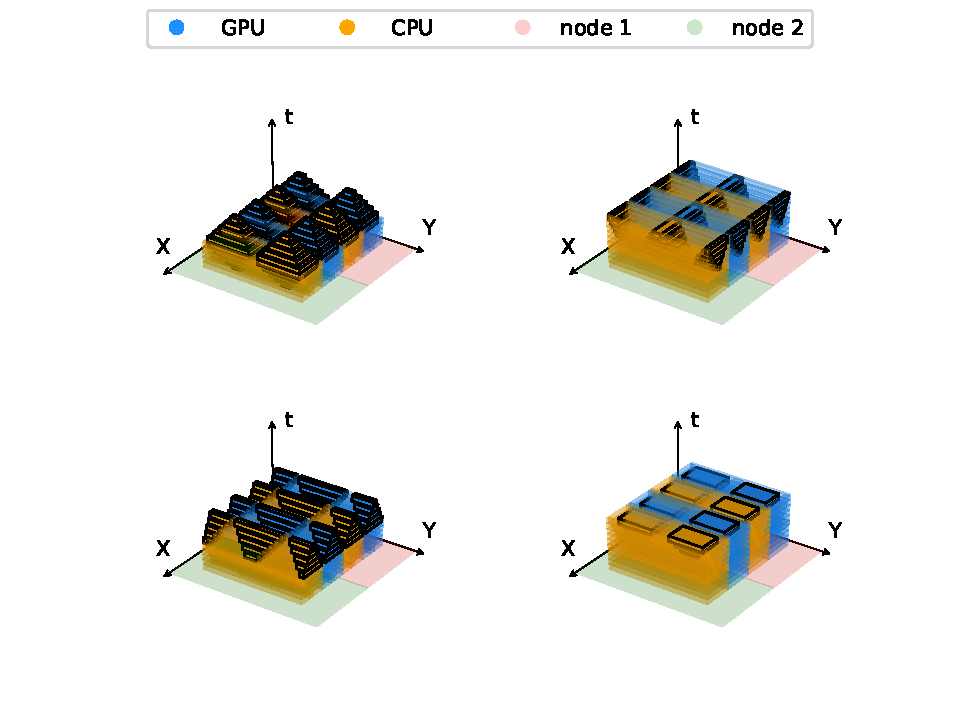
\includegraphics[height=9cm,width=0.78\textwidth, trim={1cm 0.6cm 0.25cm 0.2cm},clip]{figs/SubsPlot1.pdf}
    \end{center}
    \caption{The first four steps in the swept solution process: \Up{} (top left), \Yb{} (top right), \texttt{Communication} (bottom left), and \Xb{} (bottom right).}
    \label{fig:MainOne}
\end{figure}

\par
Depending on the decomposition strategy, a large portion of the Bridges can occur prior to inter-node communication. In this implementation, the \Yb{}---shown in Figure \ref{fig:MainOne} (top right)---occurs prior to the first communication. The first inter-node communication then follows by shifting nodal data $b/2$ points in the positive $x$ direction. Any data that exceeds the boundaries of its respective shared array is communicated to the appropriate adjacent node. This process is demonstrated in Figure~\ref{fig:MainOne} (bottom left). The shift in data allows previously determined sets and blocks to be used in the upcoming calculation phases so the \Xb{} proceeds directly after the communication as shown in Figure~\ref{fig:MainOne} (bottom right).

\par
The first three phases in the swept solution process demonstrated in Figure~\ref{fig:MainOne} are followed by the \Oct{} phase shown in Figure~\ref{fig:MainTwo} (top left). This phase is a superposition of the \Down{} and \Up{}. The \Down{}---shown in Figure~\ref{fig:MainTwo} (bottom right)--begins with boundaries that are $2n$ wide and expand by $2n$ on each boundary with every passing time step. This start is a natural consequence of removing these points during the \Up{} phase. The \Down{} completes upon reaching the top of the previous \Up{} or \Oct{} when the upward portion of \Oct{} phase begins. The entire \Oct{} is calculated in the same fashion as the \Up{} on both CPUs and GPUs. While the steps are described separately for clarity, they occur in a single calculation step without communication between ranks. 

\par
The \Oct{} always precedes the \Yb{}, Communicate, \Xb{} sequence. However, the communication varies in direction as the shift and communication of data is always the opposite of the former communication. We repeated this series of events as many times as was necessary to reach the final desired time of each simulation. The final phase is the aforementioned \Down{} which occurs only once at the end of the simulation. We show the ending sequence---minus the communication---in its entirety in Figure~\ref{fig:MainTwo}. 

% Octahedron

\begin{figure}[H]
    \begin{center}
        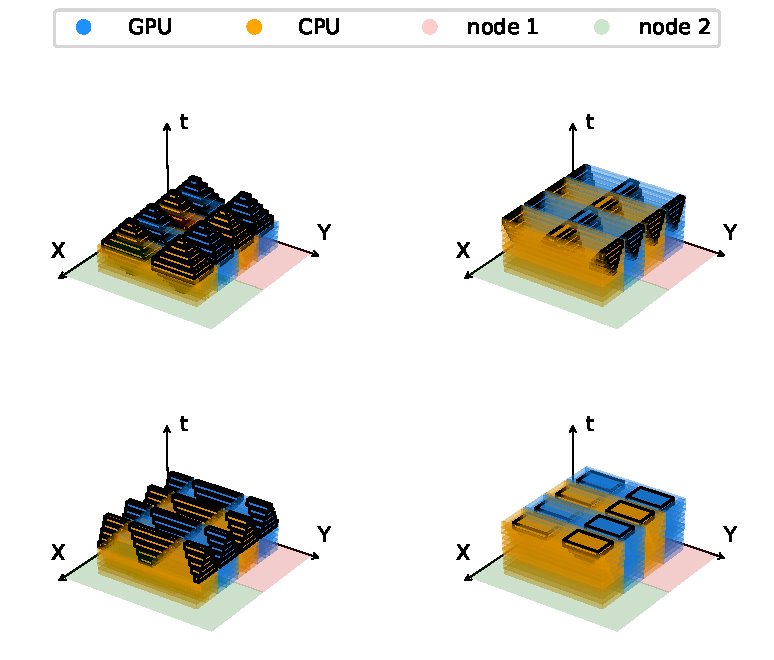
\includegraphics[height=9cm,width=0.78\textwidth, trim={1cm 0.6cm 0.25cm 0cm},clip]{figs/SubsPlot2.pdf}
    \end{center}
    \caption{The intermediate and final steps of the swept solution: \Oct{} (top left), \Xb{} (top right), \Yb (bottom left), and \Down{} (bottom right).}
    \label{fig:MainTwo}
\end{figure}

\par
The final number of time steps taken by a swept simulation is determined by the number of \Oct{} phases ($2(k-1)$ time steps) that most accurately capture the specified number of time steps. This is a consequence of the swept rule: the exact number of steps is not always achievable in some cases because the simulation only stops after the completion of a phase. These phases occur on both the GPU and CPU with respect to the given share. Between each calculation step, a communication step occurs that consists of shared memory data management and writing to disk.

\par The shared-memory data management of the communication step as well as the writing to disk involve a couple of nuances worth mentioning. It includes shifting the data, which is a strategy implemented for handling boundary blocks in the array. \pysweep{} was implemented with periodic boundary conditions based on the targeted test problems. The boundary blocks of the array form half of the shape it would normally form in the direction orthogonal to the boundary (e.g., during the \Oct{} phase on the boundary where $x=0$, only half the \Oct{} will be formed in the $x$ direction). As expected, the corner will form a fourth of the respective shape. In lieu of added logic for handling these varying shapes, we implemented a data shifting strategy that allows the majority of the same functions and kernels to be used. The boundary points are able to be solved as if they were in the center of a block with this strategy. This strategy comes at the expense of moving the data in memory. 

\par \pysweep{} writes to disk during every communication as it is the ideal time. The code uses parallel HDF5 (h5py) so that each rank can write its data to disk independently of other ranks \cite{Collette2008HDF5Python}. The size of the shared memory array is $2(k-1)$ spaces in time plus the number of intermediate steps of the time scheme so that the intermediate steps of the scheme may be used for future steps if necessary. The appropriate fully solved steps are written to disk. The data is then moved down in the time dimension of the array so that the next phase can be calculated in the existing space.

\par
The solver has a few restrictions based on architecture and implementation which have been previously described. It is currently implemented for periodic boundary conditions but can be modified to suit other conditions using the same strategy. The solver is also capable of handling given CPU functions and GPU kernels so that it may be used for any desired application that falls within the guidelines presented here. In this condition, we found it suitable for this study.

\section{Results}
\label{results-section}

Here we present the results of applying \pysweep{} to the heat transfer and compressible flow problems introduced in section~\ref{methods-section}. When solving these problems, we varied the following parameters to assess performance: array size, block size, share, and hardware. Array sizes of [320, 480, 640, 800, 960, 1120] were used to make the total number of points span a couple orders of magnitude. Block sizes of [8, 12, 16, 24, 32] were used based on hardware constraints. Share was varied from 0 to 100\% at intervals of 10\%. Along with these parameters, we advanced each problem 500 time steps.

\subsection{Heat Diffusion Equation}
\label{hdeResults}
We solved the heat diffusion equation numerically using forward-Euler and a three-point central difference in space. We verified it against an analytical solution developed for the two-dimensional heat diffusion equation with periodic boundary conditions---the problem formulation described in Appendix~\ref{Heat-Diffusion}. Figure~\ref{fig:heatSurface} compares the temperature distribution of the numerical and analytical solutions over time. The temperature distribution is representative of a flat plate with a checkerboard pattern of hot and cold spots. We see these spots diffuse out over time and approach a steady intermediate temperature which is expected. We also see that the numerical solution matches the analytical solution which verifies that we are solving the problem correctly.

\begin{figure}[H]
    \begin{center}
        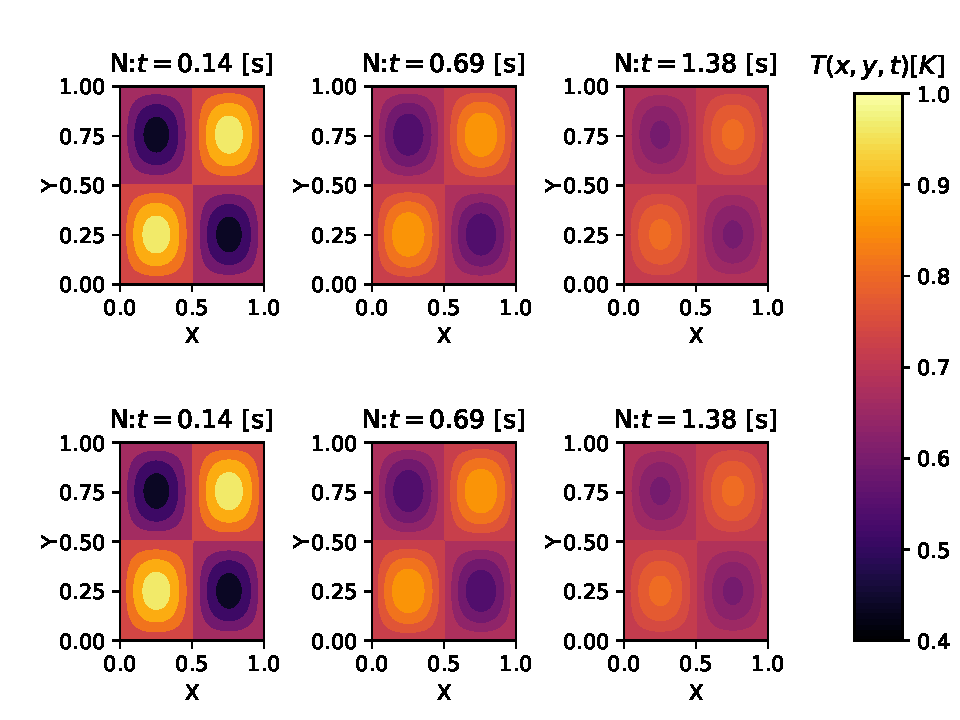
\includegraphics[height=9cm,width=0.78\textwidth, trim={0.9cm 0.3cm 0.1cm 0.9cm},clip]{figs/heatValidate.pdf}
    \end{center}
    \caption{Heat equation contours over 2000 time steps}
    \label{fig:heatSurface}
\end{figure}

Our performance metric of choice for the swept rule was speedup, $S$, as a function of array size, block size, and share. It was calculated based on the run time, $R_i$, of a simulation $i$ as
\begin{equation}
    S = \frac{R_{\textit{standard}}}{R_{\textit{swept}}}.
\end{equation}
Figures~\ref{fig:newSpeedupHeat} and~\ref{fig:oldSpeedupHeat} show the performance results produced from our tests for the two sets of hardware described in section~\ref{parameters-section}. 
Figure~\ref{fig:heatHardwareComp} shows a third contour of speedup to compare the performance across the differing hardware. This speedup is found as $R_{\textit{swept,2}}/R_{\textit{swept,1}}$. In these figures, a black dot with a white border represents the worst case and a white dot with a black border represents the best case.

\begin{figure}[H]
    
    \begin{center}
        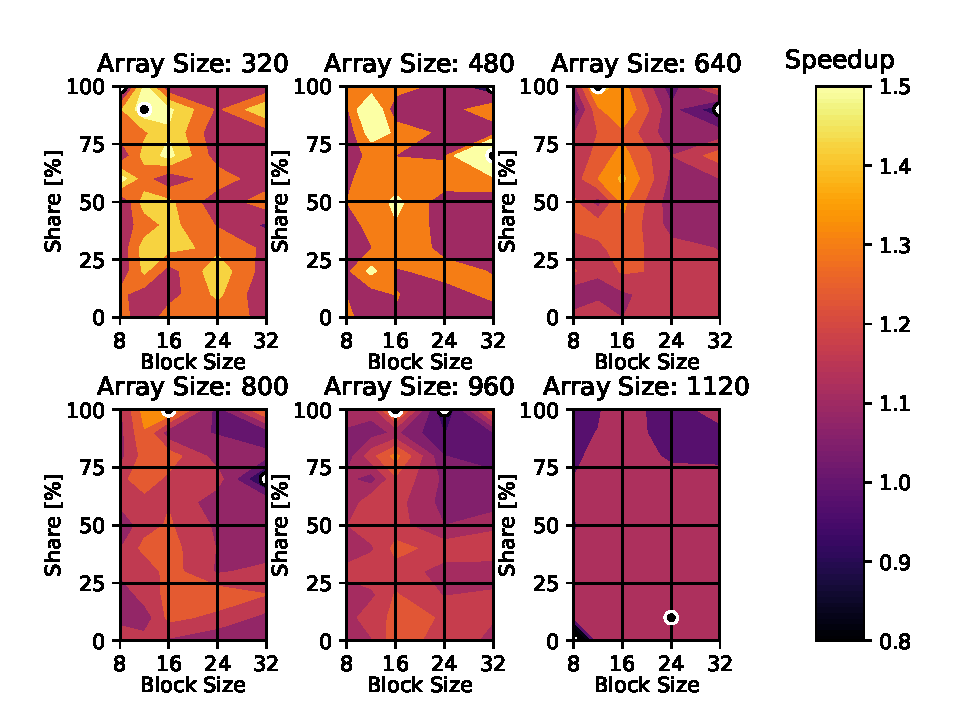
\includegraphics[height=9cm,width=0.78\textwidth, trim={0.75cm 0.4cm 0.8cm 0.7cm},clip]{figs/speedUpheatNew.pdf}
        \caption{Swept rule speedup results for the Heat Diffusion Equation with \newGPU{} GPUs and \newCPU{} CPUs.}
        \label{fig:newSpeedupHeat}
    \end{center}
\end{figure}




Figure~\ref{fig:newSpeedupHeat} shows an average speedup of 1.19. It is clear that the performance of the swept rule diminishes as the array size increases. The largest areas of performance increases generally exist above a share of 50\% and along the block size of 12-20. The majority of best cases lie between 90-100\% share and the 12-20 block size range. The worst performing cases lie close to the optimal cases: between 90-100\% share but outside the block size limits 12-20.


\begin{figure}[H]
    
    \begin{center}
        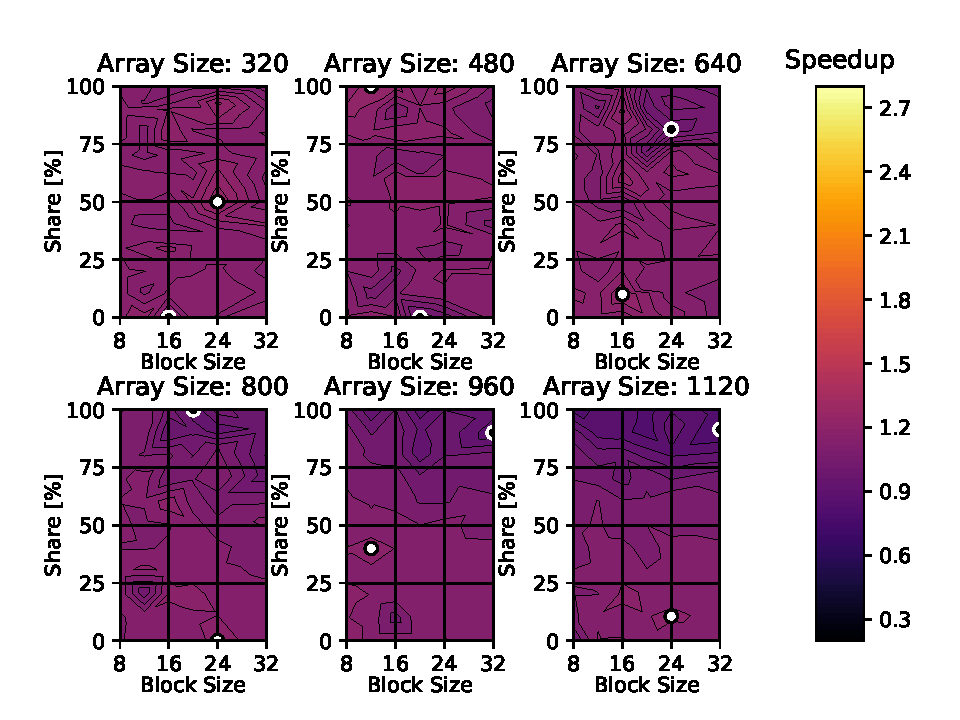
\includegraphics[height=9cm,width=0.78\textwidth, trim={0.75cm 0.4cm 0.8cm 0.7cm},clip]{figs/speedUpheatOld.pdf}
        \caption{Swept rule speedup results for the Heat Diffusion Equation with \oldGPU{} GPUs and \oldCPU{} CPUs.}
        \label{fig:oldSpeedupHeat} 
    \end{center}
\end{figure}


In Figure~\ref{fig:oldSpeedupHeat}, we see different trends than in Figure~\ref{fig:newSpeedupHeat} with an average speedup of 1.11. Performance again diminishes as array size increases, it is better with lower shares in the case of this hardware, and it somewhat consistent across different block sizes. The best case for a given array size tend to occur at or below a 50\% share and between block sizes 12-24. The worst case for a given array size tend to occur between 80-100\% share and between block sizes of 20-32 with a couple occurences on the upper limit.

\subsection{Compressible Euler Equations}
\label{eulerVortexResults}
We solved the Euler equations using a second-order Runge-Kutta in time and a five-point central difference in space with a minmod flux limiter and Roe-approximate Riemann solver, which we verified against the analytical solution to the isentropic Euler Vortex \cite{SpiegelAMethods}.

The same tests that we performed in Section~\ref{hdeResults} were repeated here. The performance results produced by these simulations are shown in Figures~\ref{fig:newSpeedupEuler} and~\ref{fig:oldSpeedupEuler} for the two sets of hardware as described in section~\ref{parameters-section}. A third contour of speedup is shown in Figure~\ref{fig:eulerHardwareComp} to compare the performance across the differing hardware. The numerical and analytical solutions are graphically compared in Figure~\ref{fig:eulerSurface}. The differences in this case are less apparent than in Figure~\ref{fig:heatSurface} but, they behave as expected. 


\begin{figure}[H]
    
    \begin{center}
       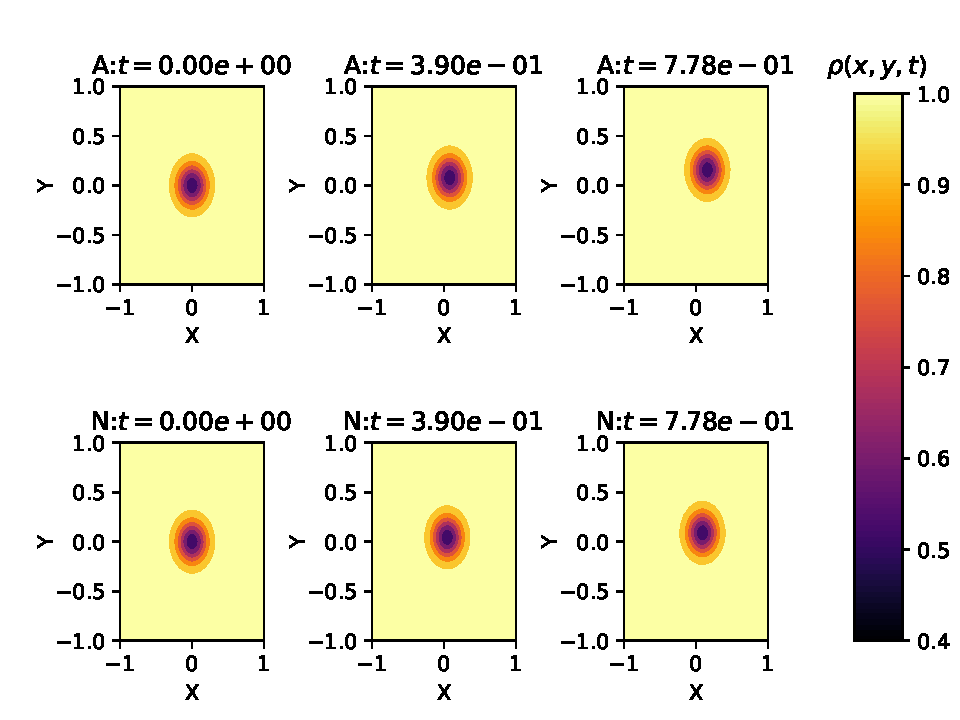
\includegraphics[height=9cm,width=0.78\textwidth, trim={0.75cm 0.3cm 0.2cm 0.2cm},clip]{figs/eulerValidate.pdf}
    \caption{Euler equations contours over 500 time steps}
    \label{fig:eulerSurface} 
    \end{center}
\end{figure}




The first hardware set results, Figure~\ref{fig:newSpeedupEuler}, show that the \Swept{} solver is consistently slower than \Standard{} with an average speedup of 0.95. Similar to the heat equation, performance declines with increasing array size but there is benefit in some cases. The majority of the best cases occur above approximately 90\% share but there is no clear block size trend. The majority of the worst cases occur at 100\% share but likewise a block size trend is unclear. However, in the three largest array sizes they always occur at 100\% share with a block size of 8.


\begin{figure}[H]
    
    \begin{center}
        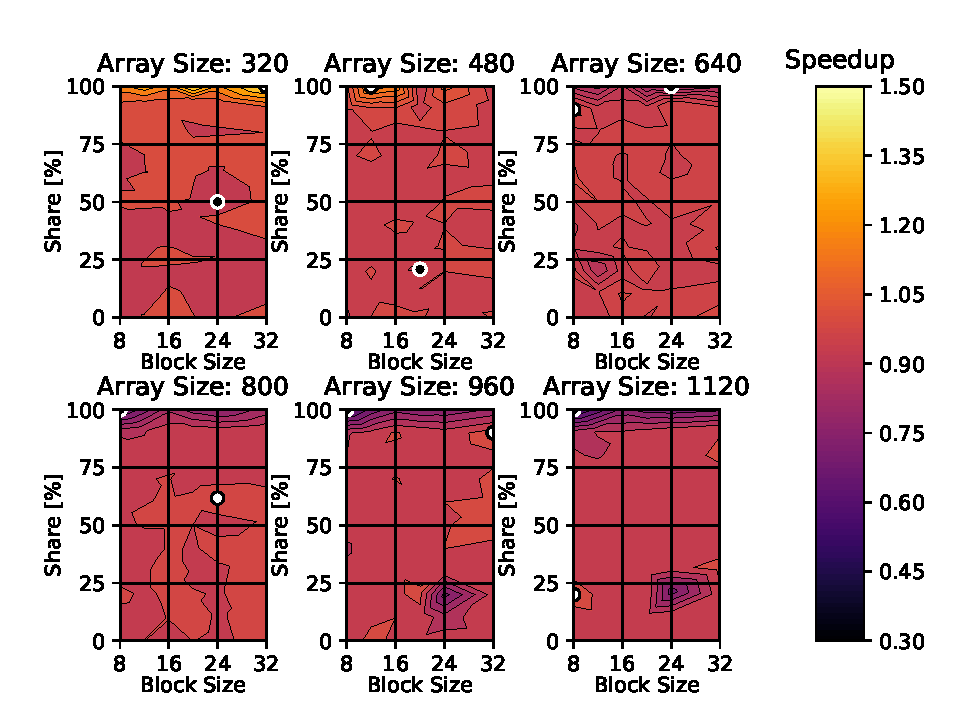
\includegraphics[height=9cm,width=0.78\textwidth, trim={0.75cm 0.4cm 0.8cm 0.7cm},clip]{figs/speedUpeulerNew.pdf}
        \caption{Swept rule speedup results  for the compressible Euler equations with \newGPU{} GPUs and \newCPU{} CPUs.}
        \label{fig:newSpeedupEuler}
    \end{center}
\end{figure}




The second hardware set results, Figure~\ref{fig:oldSpeedupEuler}, show that the \Swept{} solver is consistently slower than \Standard{} with an average speedup of 0.94. Again, performance declines with increasing array size but there is benefit in some cases. The majority of the best cases occur below approximately 50\% share with a block size between 12-24. The majority of the worst cases occur at 100\% share on the block size limits of 8 and 32.


\begin{figure}[H]
    
    \begin{center}
        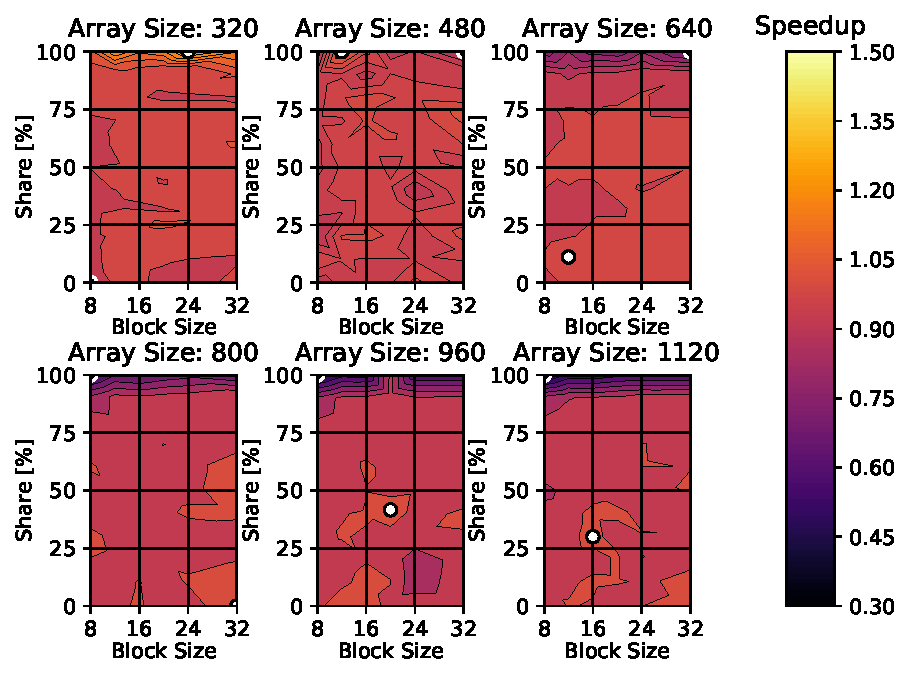
\includegraphics[height=9cm,width=0.78\textwidth, trim={0.75cm 0.4cm 0.8cm 0.7cm},clip]{figs/speedUpeulerOld.pdf}
        \caption{Swept rule speedup results  for the compressible Euler equations with \oldGPU{} GPUs and \oldCPU{} CPUs.}
        \label{fig:oldSpeedupEuler}
    \end{center}
\end{figure}




Figure~\ref{fig:eulerHardwareComp} shows the comparison between the two hardware sets for the \Swept{} solver. On average, the first set of hardware is slower than the second with an average speedup of 0.95. Set one's best speedup is 1.50 and its worst is 0.73. There are however regions in which performance benefits of the first set are evident. Shares above 90\% across most block sizes and array sizes are evidence of this. Otherwise, the results are worse. 

\begin{figure}[H]
    
    \begin{center}
        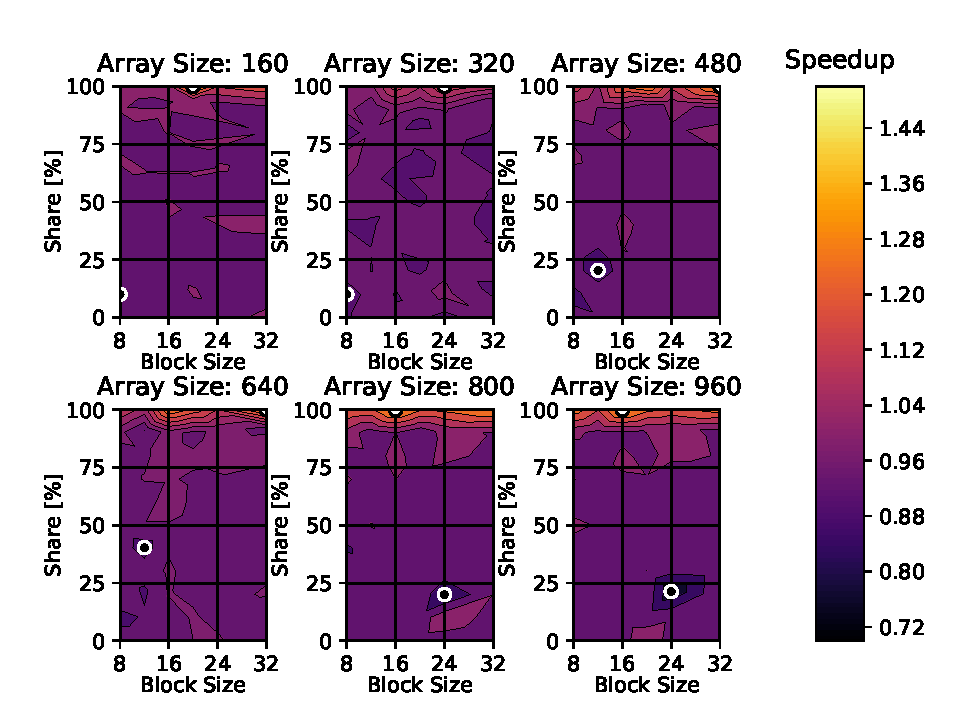
\includegraphics[height=9cm,width=0.78\textwidth, trim={0.75cm 0.4cm 0.8cm 0.7cm},clip]{figs/hardwareSpeedUpeuler.pdf}
        \caption{\Swept{} hardware speedup comparison for the Euler equations.}
        \label{fig:eulerHardwareComp}
    \end{center}
\end{figure}

\begin{figure}[H]
    
    \begin{center}
        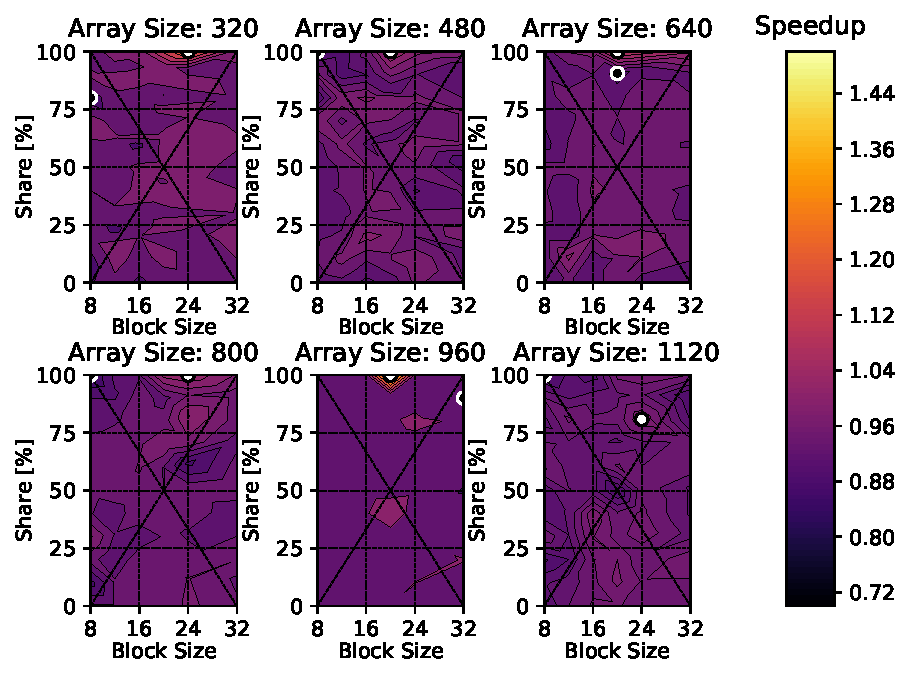
\includegraphics[height=9cm,width=0.78\textwidth, trim={0.75cm 0.4cm 0.8cm 0.7cm},clip]{figs/hardwareStandardSpeedUpeuler.pdf}
        \caption{\Standard{} hardware speedup comparison for the Euler equations.}
        \label{fig:eulerHardwareCompStd}
    \end{center}
\end{figure}


\subsection{Weak-scalability}
These results raised some questions about the performance, e.g., why the swept rule performance decreases with increasing array size. We considered the weak-scalability of the algorithms to explore this. Figure~\ref{fig:scalability} shows that the \Standard{} solver has better weak-scalability than \Swept{} for both problems. However, the slope is more shallow for the heat diffusion equation than it is for the Euler equations. 

\begin{figure}[H]
    
    \begin{center}
        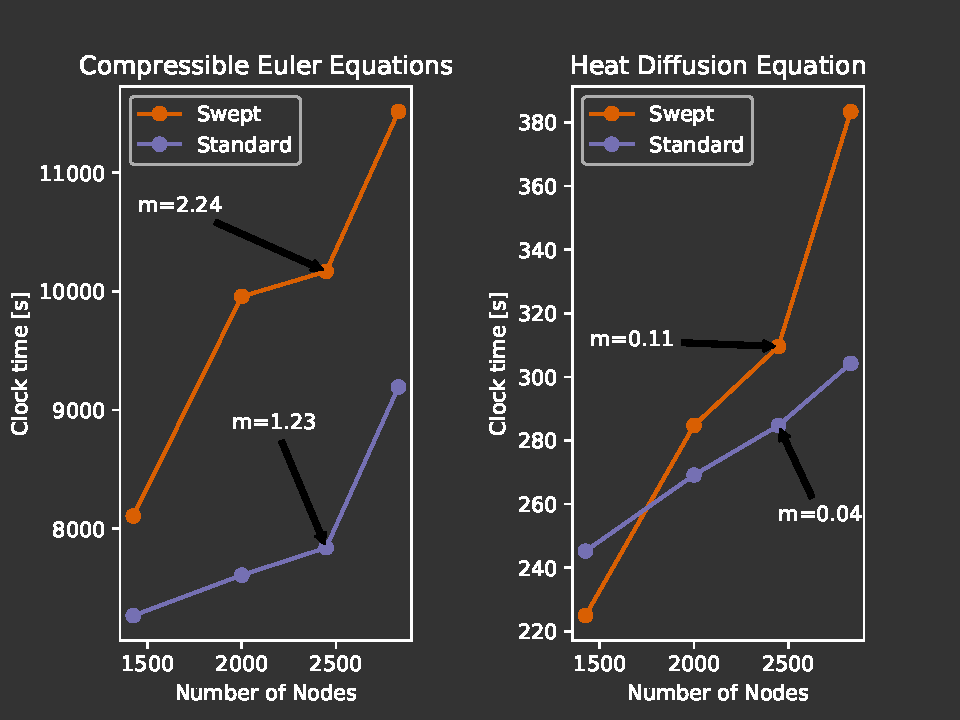
\includegraphics[height=9cm,width=0.78\textwidth, trim={0.1cm 0.25cm 1cm 0.5cm},clip]{figs/weakScalability.pdf}
        \caption{Weak-scalability of the \Swept{} and \Standard{} algorithms.}
        \label{fig:scalability}
    \end{center}
\end{figure}




\section{Discussion}
\label{discussion-section}
In regards to the heat diffusion equation, we see an overall range of speedup from 0.22-2.71 for the first hardware set and 0.79-1.32 for the second. However the limits of speedup seem to be outliers. These speedups pale in comparison to the one-dimensional heterogeneous version which reported 1.9 to 23 times speedup and, the one-dimensional GPU version which reported 2 to 9 times speedup for similar applications for the  \cite{Magee2018AcceleratingDecomposition,Magee2020ApplyingSystems}. 

For the Euler equations, we see an overall range of 0.52-1.46 for the first set of hardware and 0.36-1.42 for the second. These speedups are better aligned with values reported in other studies. The two-dimensional CPU version reported a speedup of at most 4, the one-dimensional GPU version reported 0.53-0.83, and the one-dimensional heterogeneous version reported 1.1-2.0 \cite{Alhubail2018ThePDEs,Magee2018AcceleratingDecomposition,Magee2020ApplyingSystems}.

It is consistent between studies that the swept rule performance declines as numerical complexity increases. We suspect that the magnitude of speedups differ noticeably because performance seems to be heavily tied to the implementation. This implementation relied heavily on Python which is interpretive and generally slower than C++ or other compiled languages.  

From these results, we believe that the swept rule can be helpful or harmful to simulation performance but testing is required to see which is the case. It depends on the problem solved, desired numerical scheme, and implementation used. It is also hardware dependent as is seen in Figures~\ref{fig:heatHardwareComp} and~\ref{fig:eulerHardwareComp}. It will not be suited for all numerical schemes especially those that are more complicated and cannot be parallelized well. We do believe, however, that optimizations can be made to obtain better performance in general. 

One optimization in the right direction is that of the communication step. The deterioration of performance as array size is increased is connected to the implementation of the communication step of the \Swept{} solver. We believe this issue can in part be corrected by changing the communication strategy. Currently, the dynamic programming approach considers the data and perspective of the data as if each process is looking at a certain portion. The process perspective is fixed and data is moved such that the swept solution can proceed in a simple manner. If we converted the algorithm such that the perspective is moved and not the data, we should see better performance in this regard.

The scalability results also suggest that something other than latency is more dominant in the swept rule implementation because ideally the swept rule would scale better having less latency from communication. We suspect that the implementation of the communication step of the \Swept{} solver is the cause of this. This suspicion is supported by the difference in scalability between the two cases. During the communication step, some of the data transferred is not necessary for the calculation steps which leads us to believe that bandwidth is dominating the communication. The Euler equations have quite a bit more data to communicate and thus would perform worse in this case. Larger amounts of data when solving these equations also contributes to deterioration of performance as the array size increases. The communication of unnecessary data could be corrected but it would involve some more complicated logic which may or may not yield performance benefits.

Other causes of poor performance could be steps that the \Swept{} solver takes but the \Standard{} does not. \pysweep{} determines and stores the appropriate blocks for communication prior to the simulation to avoid conditionals with the intention of boosting GPU performance. This process was parallelized as much as possible but there are some serial parts which undoubtedly reduce the performance of the algorithm. 

Scalability and array size aside, performance is also tied to the block size. It is interesting that the best case frequently occurs between lower block sizes because the block size directly limits the number of steps that can be taken prior to a communication. So, we originally expected better performance with larger block sizes but this is not necessarily the case in all the tests. We believe this could be the result of the bandwidth expense dominating the simulation. If that is the case, this would also improve with the aforementioned optimizations.


\begin{figure}[H]
    
    \begin{center}
        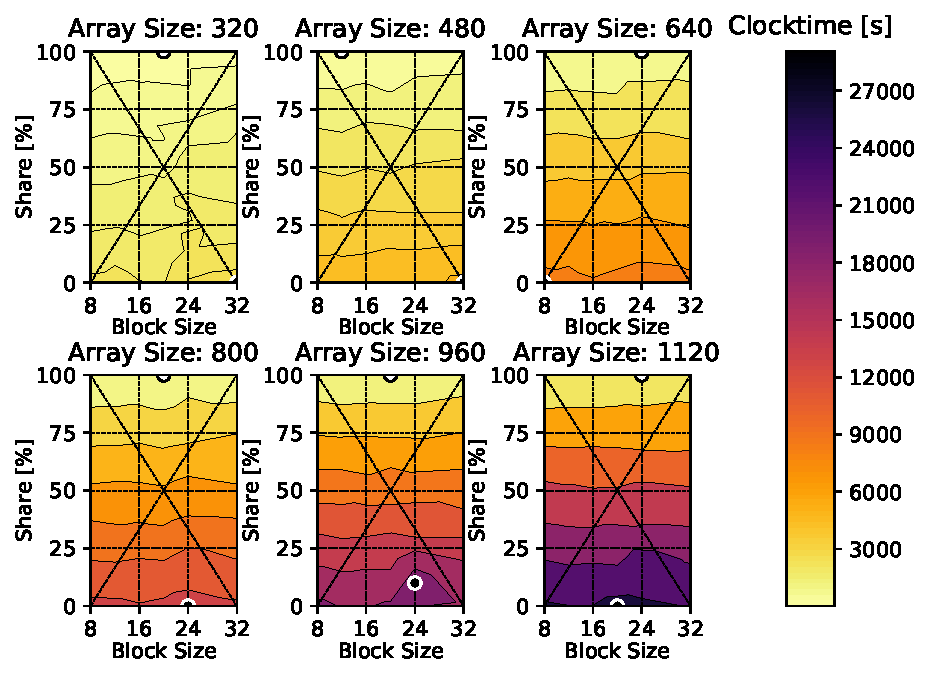
\includegraphics[height=9cm,width=0.78\textwidth, trim={0.5cm 0.4cm 0.5cm 0.2cm},clip]{figs/clockTimeSwepteulerOld.pdf}
        \caption{Clock time results  for the compressible Euler equations with \oldGPU{} GPUs and \oldCPU{} CPUs.}
        \label{fig:clocktimeOldEuler}
    \end{center}
\end{figure}



The fastest option is typically the most desired outcome when it comes to high performance computing applications. While in some cases a GPU share of less than 100\% yield faster results, this is not one of those cases. Figure~\ref{fig:clocktimeOldEuler} demonstrates that the clock time only increases as share decreases. Note, figures for clock time in other cases were not presented because they show the same result---100\% has the lowest clock time. However, the optimal configuration is useful if simulation requires data greater than the limit of the GPU(s). We expected that higher values of share would typically yield the best results but that was not necessarily the case. The first set of hardware followed this trend but the second set did the opposite. 

%%%%%%%%%%%%%%%%%%%%%%%%%%%%%%%%%%%%%%%%%%
\section{Conclusions}

\label{conclusions-section}
\pysweep{} is a two-dimensional implementation of the swept rule on heterogeneous architecture. It was tested over an array of GPU shares, block sizes, and array sizes with two hardware configurations each containing two nodes. The purpose of this study was to understand the objectives as stated in section~\ref{methods-section}.

Overall, we were able to gain insight to the performance benefits of the swept rule on distributed heterogeneous architecture. We showed that the swept rule can be both beneficial and detrimental. We believe that these benefits can be furthered by optimization but even then the performance is seemingly limited and will only be further limited with higher dimensionality and more practical numerical schemes. This is evident by the differing performance between simple schemes in not only this study but its precursors.

Next, we wanted to consider the impact of different hardware and determined that there are some substantial differences. The first set of hardware, which is newer technology, produced more speedup between the \Swept{} and \Standard{} solvers but performed worse when compared to the same solver with the other hardware set. We suspect this is because the first hardware set has nearly double the bandwidth capabilities of the second set which makes the bandwidth expense less dominant in swept communications. Better performance when comparing \Swept{} and \Standard{} for the first hardware set also supports the conclusion in section~\ref{results-section} that bandwidth is one of the dominating expenses in the current implementation.

Finally, we wanted to consider the impact of the swept performance on parameters of interest, e.g., share, block size, and array size. We considered the mode of the optimal and worst cases to further draw conclusions here. \texttt{Pysweep's} performance decreases as array size increases. This decrease in performance is a result of the implementation which can be somewhat corrected to mitigate this. The share does have an impact on shortest simulation time but does not impact the optimal configuration as much. In fact, the number of occurrences of best and worst cases were very similar for each value of share. We believe the number of occurrences are similar and share does not greatly impact the optimal configuration because of the shared memory paradigm which mitigates cost of intra-node communication. 
Configuration aside, it was always fastest to use a share of 1.

The block size greatly impacted the performance of the swept rule. We determined that the optimal cases occur most in a range of 12-24. The worst cases are an inverse of this where the greatest number of occurrences are on the boundary block sizes 8 and 32. It was expected that the largest block size would have the greatest performance and the smallest would have the worst because it limits the swept steps. However, this was not exactly the case. We believe this is a result of balancing thread occupancy and latency improvements. Smaller blocks have more communications and larger blocks have greater thread vacancy towards the end of a simulation phase. So, it makes sense that the best cases are balancing the latency savings while not completely sacrificing thread occupancy. 

We can conclude from this study that the swept rule is highly implementation dependent and it does have potential for benefit, albeit this is limited for complicated numerical schemes. As a rough heuristic, we would suggest starting with a block size of 16, a share above 80\%, and tuning to optimal performance from there. However, there are multiple cases in which the optimal performance is far from these parameters. Unfortunately, a sweep of the parameters is the best way to determine the best configuration. Finally, we believe that to optimize \pysweep{} we would need to further explore strategies for the communication step and utilize a compiled language for the core of the code to better realize the effects of the swept rule. However, this version was a good start and provided insight into the potential of the method. 

%%%%%%%%%%%%%%%%%%%%%%%%%%%%%%%%%%%%%%%%%%
\vspace{6pt} 

%%%%%%%%%%%%%%%%%%%%%%%%%%%%%%%%%%%%%%%%%%
%% optional
%\supplementary{The following are available online at \linksupplementary{s1}, Figure S1: title, Table S1: title, Video S1: title.}

% Only for the journal Methods and Protocols:
% If you wish to submit a video article, please do so with any other supplementary material.
% \supplementary{The following are available at \linksupplementary{s1}, Figure S1: title, Table S1: title, Video S1: title. A supporting video article is available at doi: link.} 


\funding{This material is based upon work supported by NASA under award No. NNX15AU66A under the technical monitoring of Drs. Eric Nielsen and Mujeeb Malik.}

\dataavailability{All code to reproduce the data can be found at \github{}}.

\acknowledgments{We gratefully acknowledge the support of NVIDIA Corporation, who donated a Tesla K40c GPU used in developing this research.}

%%%%%%%%%%%%%%%%%%%%%%%%%%%%%%%%%%%%%%%%%%
%% Optional
\appendixtitles{yes} % Leave argument "no" if all appendix headings stay EMPTY (then no dot is printed after "Appendix A"). If the appendix sections contain a heading then change the argument to "yes".
\appendixstart
\appendix
\section{Heat Diffusion Equation}
\label{Heat-Diffusion}
The heat diffusion problem is as follows:
\begin{align*}
    &\rho c_p \frac{\partial T}{\partial t} = k\frac{\partial^2 T}{\partial x^2}+k\frac{\partial^2 T}{\partial y^2},\quad 0<x<1,\quad 0<y<1,\quad t>0\\
    &T(0,y,t) = T(1,y,t),\quad 0<x<1,\quad t>0\\
    &T(x,0,t) = T(x,1,t),\quad 0<y<1,\quad t>0\\
    &T(x,y,0) = \sin(2\pi x) \sin(2\pi y) \;, \quad 0\leq x\leq 1,\quad 0 \leq y \leq 1
\end{align*}
with an analytical solution of
\begin{equation*}
\label{heat-analyt}
    T(x,y,t) = \sin(2\pi x) \sin(2\pi y) e^{-8\pi^2\alpha t}
\end{equation*}
and an update equation of 
\begin{equation*}
    \label{heat-update}
    T_{i,j}^{k+1} = T_{i,j}^{k}+\frac{\alpha \Delta t}{\Delta x^2}\big(T_{i+1,j}^{k}-2T_{i,j}^{k}+T_{i-1,j}^{k}\big)+\frac{\alpha \Delta t}{\Delta y^2}\big(T_{i,j+1}^{k}-2T_{i,j}^{k}+T_{i,j-1}^{k}\big) \;.
\end{equation*}

\section{Compressible Euler Vortex}
\label{Compressible-Euler}
The compressible Euler equations and the equation of state used are as follows where subscripts represent derivatives with respect to the spatial dimensions (x and y) or time (t).
\begin{align*}
    &\rho_t  = (\rho u)_x + (\rho v)_y \\ 
    &(\rho u)_t  = (\rho u+P)_x + (\rho u v)_y\\
    &(\rho v)_t  = (\rho v+P)_y + (\rho u v)_x\\
    &E_t = ((E+P)u)_x+((E+P)v)_y\\
    &E = \frac{P}{\gamma -1}+\frac{1}{2}\rho(u^2+v^2)
\end{align*}
The analytical solution to the isentropic Euler vortex was used as the initial conditions and in verification. The analytical solution was developed from \cite{SpiegelAMethods}. The solution is simple in the sense that it is just translation of the initial conditions. It involves superimposing perturbations in the form:
\begin{align*}
    &\delta u = -\frac{y}{R}\Omega\\
    &\delta v = -\frac{x}{R}\Omega\\
    &\delta T = -\frac{\gamma-1}{2} \Omega^2\\
    &\Omega = \beta e^{f}\text{, where } f(x,y) = -\frac{1}{2\sigma^2}\Bigg[\bigg(\frac{x}{R}^2\bigg)+\frac{y}{R}^2\bigg)\Bigg].
\end{align*}
The initial conditions are then 
\begin{align*}
    &\rho_0 = (1+\delta T)^{\frac{1}{\gamma-1}},\\
    &u_0 = M_\infty \cos(\alpha)+\delta u,\\
    &v_0 = M_\infty \sin(\alpha)+\delta v,\\
    &p_0 = \frac{1}{\gamma}(1+\delta T)^\frac{\gamma}{\gamma-1}.
\end{align*}
The specific values used are shown in Table~\ref{tab:eulerVortex}
\begin{table}[htb!]
    \centering
    \begin{tabular}{|c|c|c|c|c|c|c|c|c|}
    \hline
         $\alpha$ & $M_\infty$  & $\rho_\infty$ & $p_\infty$ & $T_\infty$ & $R$ & $\sigma$ & $\beta$ & $L$\\\hline
         $45^\circ$ &  $\sqrt{\frac{2}{\gamma}}$ & $1$ & $1$ & $1$ & $1$ & $1$ & $M_\infty \frac{5\sqrt{2}}{4\pi}e^{1/2}$ & $5$\\ \hline
    \end{tabular}
    \caption{Conditions used in analytical solution \cite{shu1998essentially}}
    \label{tab:eulerVortex}
\end{table}

Similar to the heat diffusion equation, periodic boundary conditions were implemented. The numerical scheme implemented was nearly a carbon copy of what was done in \cite{Magee2018AcceleratingDecomposition} except it was extended into two dimensions. A five point finite volume method was used in space with a minmod flux limiter and second order Runge-Kutta was used in time. Consider equations of the form
\begin{equation*}
    \frac{\partial Q}{\partial t}+\frac{\partial F}{\partial x}+\frac{\partial G}{\partial y} = 0,
\end{equation*}
where
\begin{equation*}
    Q = \begin{bmatrix}
        \rho\\
        \rho u\\
        \rho v\\
        E
        \end{bmatrix}
        \text{, }
    F = \begin{bmatrix}
    \rho u\\
    \rho u^2+p\\
    \rho u v\\
    (E+p)u
    \end{bmatrix}
    \text{ and, }
    G = \begin{bmatrix}
    \rho v\\
    \rho u v\\
    \rho v^2+p\\
    (E+p)v
    \end{bmatrix}
\end{equation*}
The pressure ratio was used in the minmod limiter to compute reconstructed values on the cell boundaries.
\begin{align*}
   & P_{r,i} = \frac{P_{i+1}-P_{i}}{P_{i}-P_{i-1}}\\
    &Q_n^{i} = \begin{cases} 
      Q_o^{i}+\frac{\min(P_{r,i}^1,1)}{2}(Q_o^{i+1)}-Q_o^{i}) & 0 < P_{r,i} < \infty \\
      Q_0^{i} \\
   \end{cases}\\
    &Q_n^{i+1} = \begin{cases} 
      Q_o^{i+1}+\frac{\min(P_{r,i+1}^{-1},1)}{2}(Q_o^{i}-Q_o^{i+1}) & 0 < P_{r,i}^{-1} < \infty \\
      Q_0^{i+1} \\
   \end{cases}
\end{align*}
The flux is then calculated with the reconstructed values for i and i+1 accordingly and used to step in time.
\begin{align*}
    &F_{i+1} = \frac{1}{2}\big( F(Q^{i+1})+F(Q^{i})+r_{x,sp}(Q^{i}-Q^{i+1})\big)\\
    &G_{i+1} = \frac{1}{2}\big( G(Q^{i+1})+G(Q^{i})+r_{y,sp}(Q^{i}-Q^{i+1})\big)\\
\end{align*}
where $r_{i,sp}$ is the spectral radius or largest eigenvalue for the appropriate Jacobian matrix. These flux calculations are then used to apply the second order Runge-Kutta in time---the process looks like
\begin{align*}
    &Q_i^{*} = Q_i^{n}+\frac{\Delta t}{2\Delta x}(F_{i+1/2}(Q^n)+F_{i-1/2}(Q^n))+\frac{\Delta t}{2\Delta y}(G_{i+1/2}(Q^n)+G_{i-1/2}(Q^n)),\\
    &Q_i^{n+1} = Q_i^{n}+\frac{\Delta t}{\Delta x}(F_{i+1/2}(Q^*)+F_{i-1/2}(Q^*))+\frac{\Delta t}{\Delta y}(G_{i+1/2}(Q^*)+G_{i-1/2}(Q^*)).
\end{align*}


\section{Hardware}
\label{Hardware}
\begin{table}[htb!]
\begin{center}
\begin{tabular}{ |c|c|c| } 

 \hline
 Hardware Specifications & Set 1 & Set 2 \\
 \hline
 GPU & \newGPU{} & \oldGPU{} \\
 Architecture   & Volta &  Pascal \\
 NVIDIA CUDA® Cores  & 5120 &  3584 \\
 Memory Type   & 32 GB HBM2 &  11 GB GDDR5X \\
 Bus Width    & 4096 bit &  352-bit \\
 Memory Bandwidth (GB/sec)  & 900 &  484 \\ 
 \hline
 CPU & \newCPU{} & \oldCPU{} \\ 
 Cores & 20 & 10 \\
 Processor Base Frequency & 2.20 GHz & 2.20 GHz \\
 Cache & 50 MB Intel® Smart Cache & 13.75 MB L3 Cache\\
 \hline
\end{tabular}
\end{center}
\caption{\label{hardwareTable} Common specifications found between hardware sets from NVIDIA's and Intel's websites \cite{Intel123550,Intel91753,GeForceGeForce,NVIDIANVIDIA}.}
\end{table}

%%%%%%%%%%%%%%%%%%%%%%%%%%%%%%%%%%%%%%%%%%
\end{paracol}
\reftitle{References}

% Please provide either the correct journal abbreviation (e.g. according to the “List of Title Word Abbreviations” http://www.issn.org/services/online-services/access-to-the-ltwa/) or the full name of the journal.
% Citations and References in Supplementary files are permitted provided that they also appear in the reference list here. 

%=====================================
% References, variant A: external bibliography
%=====================================
\externalbibliography{yes}
\bibliography{references}


% If authors have biography, please use the format below
%\section*{Short Biography of Authors}
%\bio
%{\raisebox{-0.35cm}{\includegraphics[width=3.5cm,height=5.3cm,clip,keepaspectratio]{Definitions/author1.pdf}}}
%{\textbf{Firstname Lastname} Biography of first author}
%
%\bio
%{\raisebox{-0.35cm}{\includegraphics[width=3.5cm,height=5.3cm,clip,keepaspectratio]{Definitions/author2.jpg}}}
%{\textbf{Firstname Lastname} Biography of second author}

% The following MDPI journals use author-date citation: Arts, Econometrics, Economies, Genealogy, Humanities, IJFS, JRFM, Laws, Religions, Risks, Social Sciences. For those journals, please follow the formatting guidelines on http://www.mdpi.com/authors/references
% To cite two works by the same author: \citeauthor{ref-journal-1a} (\citeyear{ref-journal-1a}, \citeyear{ref-journal-1b}). This produces: Whittaker (1967, 1975)
% To cite two works by the same author with specific pages: \citeauthor{ref-journal-3a} (\citeyear{ref-journal-3a}, p. 328; \citeyear{ref-journal-3b}, p.475). This produces: Wong (1999, p. 328; 2000, p. 475)

%%%%%%%%%%%%%%%%%%%%%%%%%%%%%%%%%%%%%%%%%%
%% for journal Sci
%\reviewreports{\\
%Reviewer 1 comments and authors’ response\\
%Reviewer 2 comments and authors’ response\\
%Reviewer 3 comments and authors’ response
%}
%%%%%%%%%%%%%%%%%%%%%%%%%%%%%%%%%%%%%%%%%%

\end{document}

